% BUSFIN 8200 -- Problem Set 1 -- Solution
% Build: cd tex && latexmk -pdf ps1_solution.tex
% Figures/tables are produced by src/*.py into output/ and included from there.

\documentclass[11pt]{article}

% ---------- Packages ----------
\usepackage[margin=1in]{geometry}
\usepackage{amsmath, amssymb, amsthm}
\usepackage{bm}
\usepackage{graphicx}
\usepackage{booktabs}
\usepackage{caption}
\usepackage{subcaption}
\usepackage{float}
\usepackage{enumitem}
\usepackage[colorlinks=true, linkcolor=blue, citecolor=blue, urlcolor=blue]{hyperref}

\graphicspath{{../output/}}

% ---------- Macros ----------
\newcommand{\E}{\mathbb{E}}
\newcommand{\Var}{\mathrm{Var}}
\newcommand{\Cov}{\mathrm{Cov}}
\newcommand{\dpr}{\mathit{dp}}   % \dp is a TeX primitive (box depth), so use \dpr
\newcommand{\dy}{\mathit{dy}}
\newcommand{\xR}{\mathit{xR}}
\newcommand{\xr}{\mathit{xr}}
\newcommand{\xy}{\mathit{xy}}
\newcommand{\xf}{\mathit{xf}}

% ---------- Title ----------
\title{BUSFIN 8200: Asset Pricing Foundations\\Problem Set 1}
\author{Joon Bae}
\date{\today}

\begin{document}
\maketitle

% =====================================================================
\section{Question 1}
% =====================================================================

\subsection{Derivation of Equations 1.1--1.3}
% TODO (Q1a): derivation starting from R_{e,t+1} = (P_{t+1} + D_{t+1}) / P_t

Throughout, a lowercase letter denotes the log of the corresponding uppercase variable,
e.g.\ $r_{t+1} = \log(R_{t+1})$, $p_t = \log(P_t)$, and $\mathit{cf}_{t+1} = \log(\mathit{CF}_{t+1})$.

\paragraph{Step 1: log return.}
Start from the definition of the gross return,
\begin{equation}
  R_{t+1} = \frac{P_{t+1} + \mathit{CF}_{t+1}}{P_t}.
  \label{eq:q1a_gross_return}
\end{equation}
Taking logs,
\begin{align}
  \log(R_{t+1})
    &= \log(P_{t+1}) - \log(P_t) + \log\!\left(1 + \frac{\mathit{CF}_{t+1}}{P_{t+1}}\right) \nonumber \\
  \Longleftrightarrow \quad
  r_{t+1}
    &= p_{t+1} - p_t + \log\!\left(1 + e^{\,\mathit{cf}_{t+1} - p_{t+1}}\right).
  \label{eq:q1a_log_return}
\end{align}

\paragraph{Step 2: first-order Taylor approximation of the log term.}
Rearranging (\ref{eq:q1a_log_return}) so that the polynomial terms are on the left-hand side
and the log term is on the right-hand side,
\begin{equation}
  r_{t+1} - p_{t+1} + p_t = \log\!\left(1 + e^{\,\mathit{cf}_{t+1} - p_{t+1}}\right).
  \label{eq:q1a_rearranged}
\end{equation}
Let $x_{t+1} = \mathit{cf}_{t+1} - p_{t+1}$. The function $\log(1 + e^{x})$ can be
approximated by a first-order Taylor expansion around a point $a$:
\begin{equation}
  \log\!\left(1 + e^{x}\right)
    \approx \log\!\left(1 + e^{a}\right) + \frac{e^{a}}{1 + e^{a}}\,(x - a),
  \label{eq:q1a_taylor}
\end{equation}
which is accurate for small enough $x - a$. The expansion point $a$ is taken to be the
time average of $\mathit{cf}_{t+1} - p_{t+1}$, which is assumed to converge to a constant,
denoted $a = \overline{\mathit{cf}} - \overline{p}$.

\paragraph{Step 3: substituting the approximation.}
Applying the Taylor approximation (\ref{eq:q1a_taylor}) to the right-hand side of
(\ref{eq:q1a_rearranged}), with $x = \mathit{cf}_{t+1} - p_{t+1}$ and
$a = \overline{\mathit{cf}} - \overline{p}$, and rearranging the terms, we obtain
\begin{equation}
  p_t = \kappa_0 + (1 - \kappa)\,\mathit{cf}_{t+1} - r_{t+1} + \kappa\, p_{t+1},
  \label{eq:q1a_price_recursion}
\end{equation}
where, as in the problem statement,
\begin{equation}
  \kappa = \frac{1}{1 + e^{\,a}}
  \qquad \text{and} \qquad
  \kappa_0 = -\log(\kappa) - (1 - \kappa)\,\log\!\left(\frac{1}{\kappa} - 1\right),
  \label{eq:q1a_kappa_def}
\end{equation}
with $a = \overline{\mathit{cf}} - \overline{p}$ the expansion point of Step 2
(the problem statement writes this average as $\overline{\dpr}$).
% NOTE: the two definitions above are copied from the problem statement (with dp-bar
% written as a). What is still missing is the derivation-side link: showing that the
% Taylor coefficients log(1+e^a) and e^a/(1+e^a) from Step 2 reduce to these kappa_0 and
% (1-kappa) after the rearrangement. STUDENT TO ADD.
% The intermediate line (after substitution, before rearranging) was also not written by
% the student; whether to display it is the student's choice.

\paragraph{Step 4: rewriting in terms of the log cash-flow--price ratio.}
Subtracting $\mathit{cf}_t$ from both sides of (\ref{eq:q1a_price_recursion}) and multiplying
both sides by $-1$, and defining
\begin{equation}
  \dpr_t := \mathit{cf}_t - p_t
  \qquad \text{and} \qquad
  \Delta \mathit{cf}_{t+1} := \mathit{cf}_{t+1} - \mathit{cf}_t,
  \label{eq:q1a_dp_def}
\end{equation}
we obtain
\begin{equation}
  \dpr_t = -\kappa_0 + \kappa\, \dpr_{t+1} + r_{t+1} - \Delta \mathit{cf}_{t+1}.
  \label{eq:q1a_dp_recursion}
\end{equation}

\paragraph{Step 5: forward substitution.}
Equation (\ref{eq:q1a_dp_recursion}) holds at every date, so shifting it one period forward,
\begin{equation}
  \dpr_{t+1} = -\kappa_0 + \kappa\, \dpr_{t+2} + r_{t+2} - \Delta \mathit{cf}_{t+2}.
  \label{eq:q1a_dp_recursion_t1}
\end{equation}
Plugging (\ref{eq:q1a_dp_recursion_t1}) into the $\dpr_{t+1}$ term on the right-hand side of
(\ref{eq:q1a_dp_recursion}) gives
\begin{equation}
  \dpr_t = -\kappa_0 - \kappa\,\kappa_0 + \kappa^{2}\, \dpr_{t+2}
           + r_{t+1} + \kappa\, r_{t+2}
           - \Delta \mathit{cf}_{t+1} - \kappa\, \Delta \mathit{cf}_{t+2}.
  \label{eq:q1a_two_step}
\end{equation}

\paragraph{Step 6: substitution up to horizon $H$.}
Continuing to substitute the future $\dpr$ terms into (\ref{eq:q1a_two_step}) up to
horizon $H$, we get
\begin{equation}
  \dpr_t = -\kappa_0 \sum_{h=0}^{H-1} \kappa^{h}
           + \kappa^{H}\, \dpr_{t+H}
           + \sum_{h=1}^{H} \kappa^{h-1}\, r_{t+h}
           - \sum_{h=1}^{H} \kappa^{h-1}\, \Delta \mathit{cf}_{t+h}.
  \label{eq:q1a_H_step}
\end{equation}
% STUDENT TO ADD: closed form of the constant term via the finite geometric series, so
% that (\ref{eq:q1a_H_step}) matches Equation 1.1 of the problem statement, whose constant
% is kappa_0 (kappa^H - 1) / (1 - kappa).

\subsection{Variance decomposition by horizon (data)}
% TODO (Q1b): figure H vs (b_re^(H), b_dd^(H), b_dp^(H)) + inference
% \begin{figure}[H]
%   \centering
%   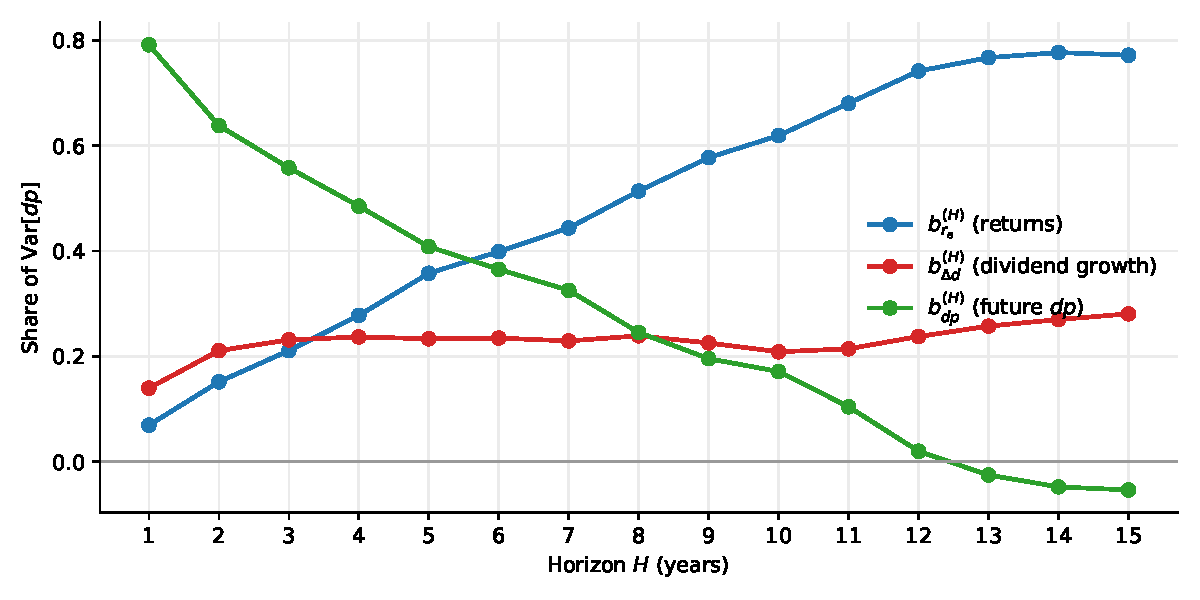
\includegraphics[width=0.8\textwidth]{q1b_decomposition.pdf}
%   \caption{}
%   \label{fig:q1b}
% \end{figure}

\subsection{Variance decomposition by horizon (VAR-implied)}
% TODO (Q1c): VAR z_{t+1} = Gamma_0 + Gamma z_t + e_{t+1}, z_t = [dd_t, r_{e,t}, dp_t]
% \begin{figure}[H] ... q1c_decomposition_var.pdf ... \end{figure}

\subsection{Infinite-horizon decomposition}
% TODO (Q1d): b_re^(inf), b_dd^(inf) from the VAR + interpretation

\subsection{Derivation of Equations 1.7--1.9 (Gao and Martin, 2021)}
% TODO (Q1e): derivation with dy_t = log(1 + D_t/P_t), kappa = e^{-dy}

% =====================================================================
\section{Question 2}
% =====================================================================

\subsection{Predictive regressions by horizon}
% TODO (Q2a): figure H vs adjusted R^2, H = 1..15 + description
% \begin{figure}[H] ... q2a_r2adj.pdf ... \end{figure}

\subsection{Standard errors for the one-year predictive regression}
% TODO (Q2b): table with b-hat and t-stats under OLS / White / NW(11) / HH(11) / NW(1994)
% \begin{table}[H]
%   \centering
%   \begin{tabular}{lccc}
\toprule
Standard-error method & SE$(\hat b)$ & $t(\hat b)$ & Lags \\
\midrule
(i) OLS & 0.3802 & 7.38 & -- \\
(ii) White (1980) & 0.6587 & 4.26 & -- \\
(iii) Newey-West (1987), 11 lags & 1.2979 & 2.16 & 11 \\
(iv) Hansen-Hodrick (1980), 11 lags & 1.4521 & 1.93 & 11 \\
(v) Newey-West (1987, 1994), automatic lags & 1.2311 & 2.28 & 24 \\
\midrule
\multicolumn{4}{l}{$\hat a = -0.0314$, \quad $\hat b = 2.8038$, \quad $T = 1117$ monthly observations} \\
\bottomrule
\end{tabular}

%   \caption{}
%   \label{tab:q2b}
% \end{table}

\subsection{Amihud and Hurvich (2004) bias-corrected estimate}
% TODO (Q2c): report b-hat, contrast with Q2b, explain why they differ

\subsection{Out-of-sample estimation (expanding window)}
% TODO (Q2d): time-series plot of xRbar, E^IS, E^OS from 1940-12; R^2_OS; 50-year rolling R^2_OS plot
% \begin{figure}[H] ... q2d_forecasts.pdf ... \end{figure}
% \begin{figure}[H] ... q2d_r2os_rolling.pdf ... \end{figure}

\subsection{Out-of-sample estimation with steady-state restrictions}
% TODO (Q2e): same as Q2d with a_t = G_t - 1, b_t = G_t
% \begin{figure}[H] ... q2e_forecasts.pdf ... \end{figure}
% \begin{figure}[H] ... q2e_r2os_rolling.pdf ... \end{figure}

% =====================================================================
\section{Question 3}
% =====================================================================

\subsection{Momentum signal construction and validation}
% TODO (Q3a): three time-series plots (intercept, slope, R^2) of MOM_CZ on MOM

\subsection{Book-to-market signal construction and validation}
% TODO (Q3b): three time-series plots (intercept, slope, R^2) of BM_CZ on BM

\subsection{Decile portfolios}
% TODO (Q3c): five scatterplots (decile vs. avg excess return; blue = BM, red = MOM, green = GP)
%             + table of 15 HML average returns with NW(1994) t-stats

\subsection{Fama--MacBeth regressions}
% TODO (Q3d): table, specifications (i)--(vii), OLS and WLS (ME weights), with t-stats

\subsection{Portfolio-level multivariate regressions}
% TODO (Q3e): table, specifications (i)--(vii), VW and EW portfolios, Driscoll--Kraay t-stats

% =====================================================================
\section{Question 4}
% =====================================================================

\subsection{Yields, forward rates, and returns}
% TODO (Q4a): table of average xy^(H), xf^(H), xr^(H) for H = 2..5

\subsection{Hold-to-maturity excess return regressions}
% TODO (Q4b): table analogous to slide 5.5, first table, first panel; Hansen--Hodrick t-stats

\subsection{One-year excess return regressions on forward spreads}
% TODO (Q4c): table analogous to slide 5.5, first table, second panel; NW(1994) t-stats

\subsection{Cochrane--Piazzesi factor}
% TODO (Q4d): time-series plot of cp_t with NBER recession shading

\subsection{Excess return regressions on the CP factor}
% TODO (Q4e): table analogous to slide 5.5, second table; NW(1994) t-stats

% =====================================================================
% \bibliographystyle{...}
% \bibliography{references}

\end{document}
